\begin{center}
 {\sffamily\small\bfseries\color{teal}AN ILLUSTRATED RESEARCH REPORT}\par\vspace{7pt}
 {\fontsize{25}{28}\selectfont\bfseries Does a moving viewpoint change\\the exoplanet sky?}\par\vspace{8pt}
 {\large A moving observer. Moving stars. Changing opportunities.}\par\vspace{9pt}
 {\large\textbf{Biswajit Jana}}\par
 {\sffamily\small Finding Earth 2.0\enspace\textbar\enspace Independent researcher and simulation author}
\end{center}
\vspace{5pt}
\textbf{The question.} As the Solar System moves through the Milky Way, could changing distances and sightlines make other planetary systems easier to detect? This report connects that curiosity to an interactive simulation and a limited, reproducible calculation. Both the observer and the target stars move; travelling farther does not by itself guarantee more discoveries.

\vspace{5pt}
\begin{minipage}[t]{.295\linewidth}\vspace{0pt}\setlength{\parskip}{3pt}
 \kicker{01 / THE ORIGINAL IDEA}
 \textbf{A: today. B: future.\\C: later future.}

 These positions illustrate a changing viewpoint along a Galactic orbit. They are epochs of the same observer, not three different stars.

 \vspace{5pt}{\fontsize{24}{26}\selectfont\color{teal}233}\enspace km/s\par
 \source{Adopted tangential speed.}

 \vspace{5pt}{\fontsize{24}{26}\selectfont\color{teal}0.0777}\enspace ly\par
 \source{Solar path in 100 years, at this speed: about 4,915 AU.}

 \vspace{5pt}{\fontsize{24}{26}\selectfont\color{teal}128,600}\par
 \source{Approximate model years needed to travel 100 light-years.}

 \vspace{8pt}\textbf{The crucial distinction}\par
 Solar travel relative to the Galaxy differs from motion relative to a nearby star. The latter changes our view of that star's planets.
\end{minipage}\hfill
\begin{minipage}[t]{.675\linewidth}\vspace{0pt}\setlength{\parskip}{3pt}
 \begin{tikzpicture}
  \node[inner sep=0,anchor=south west] (map) at (0,0) {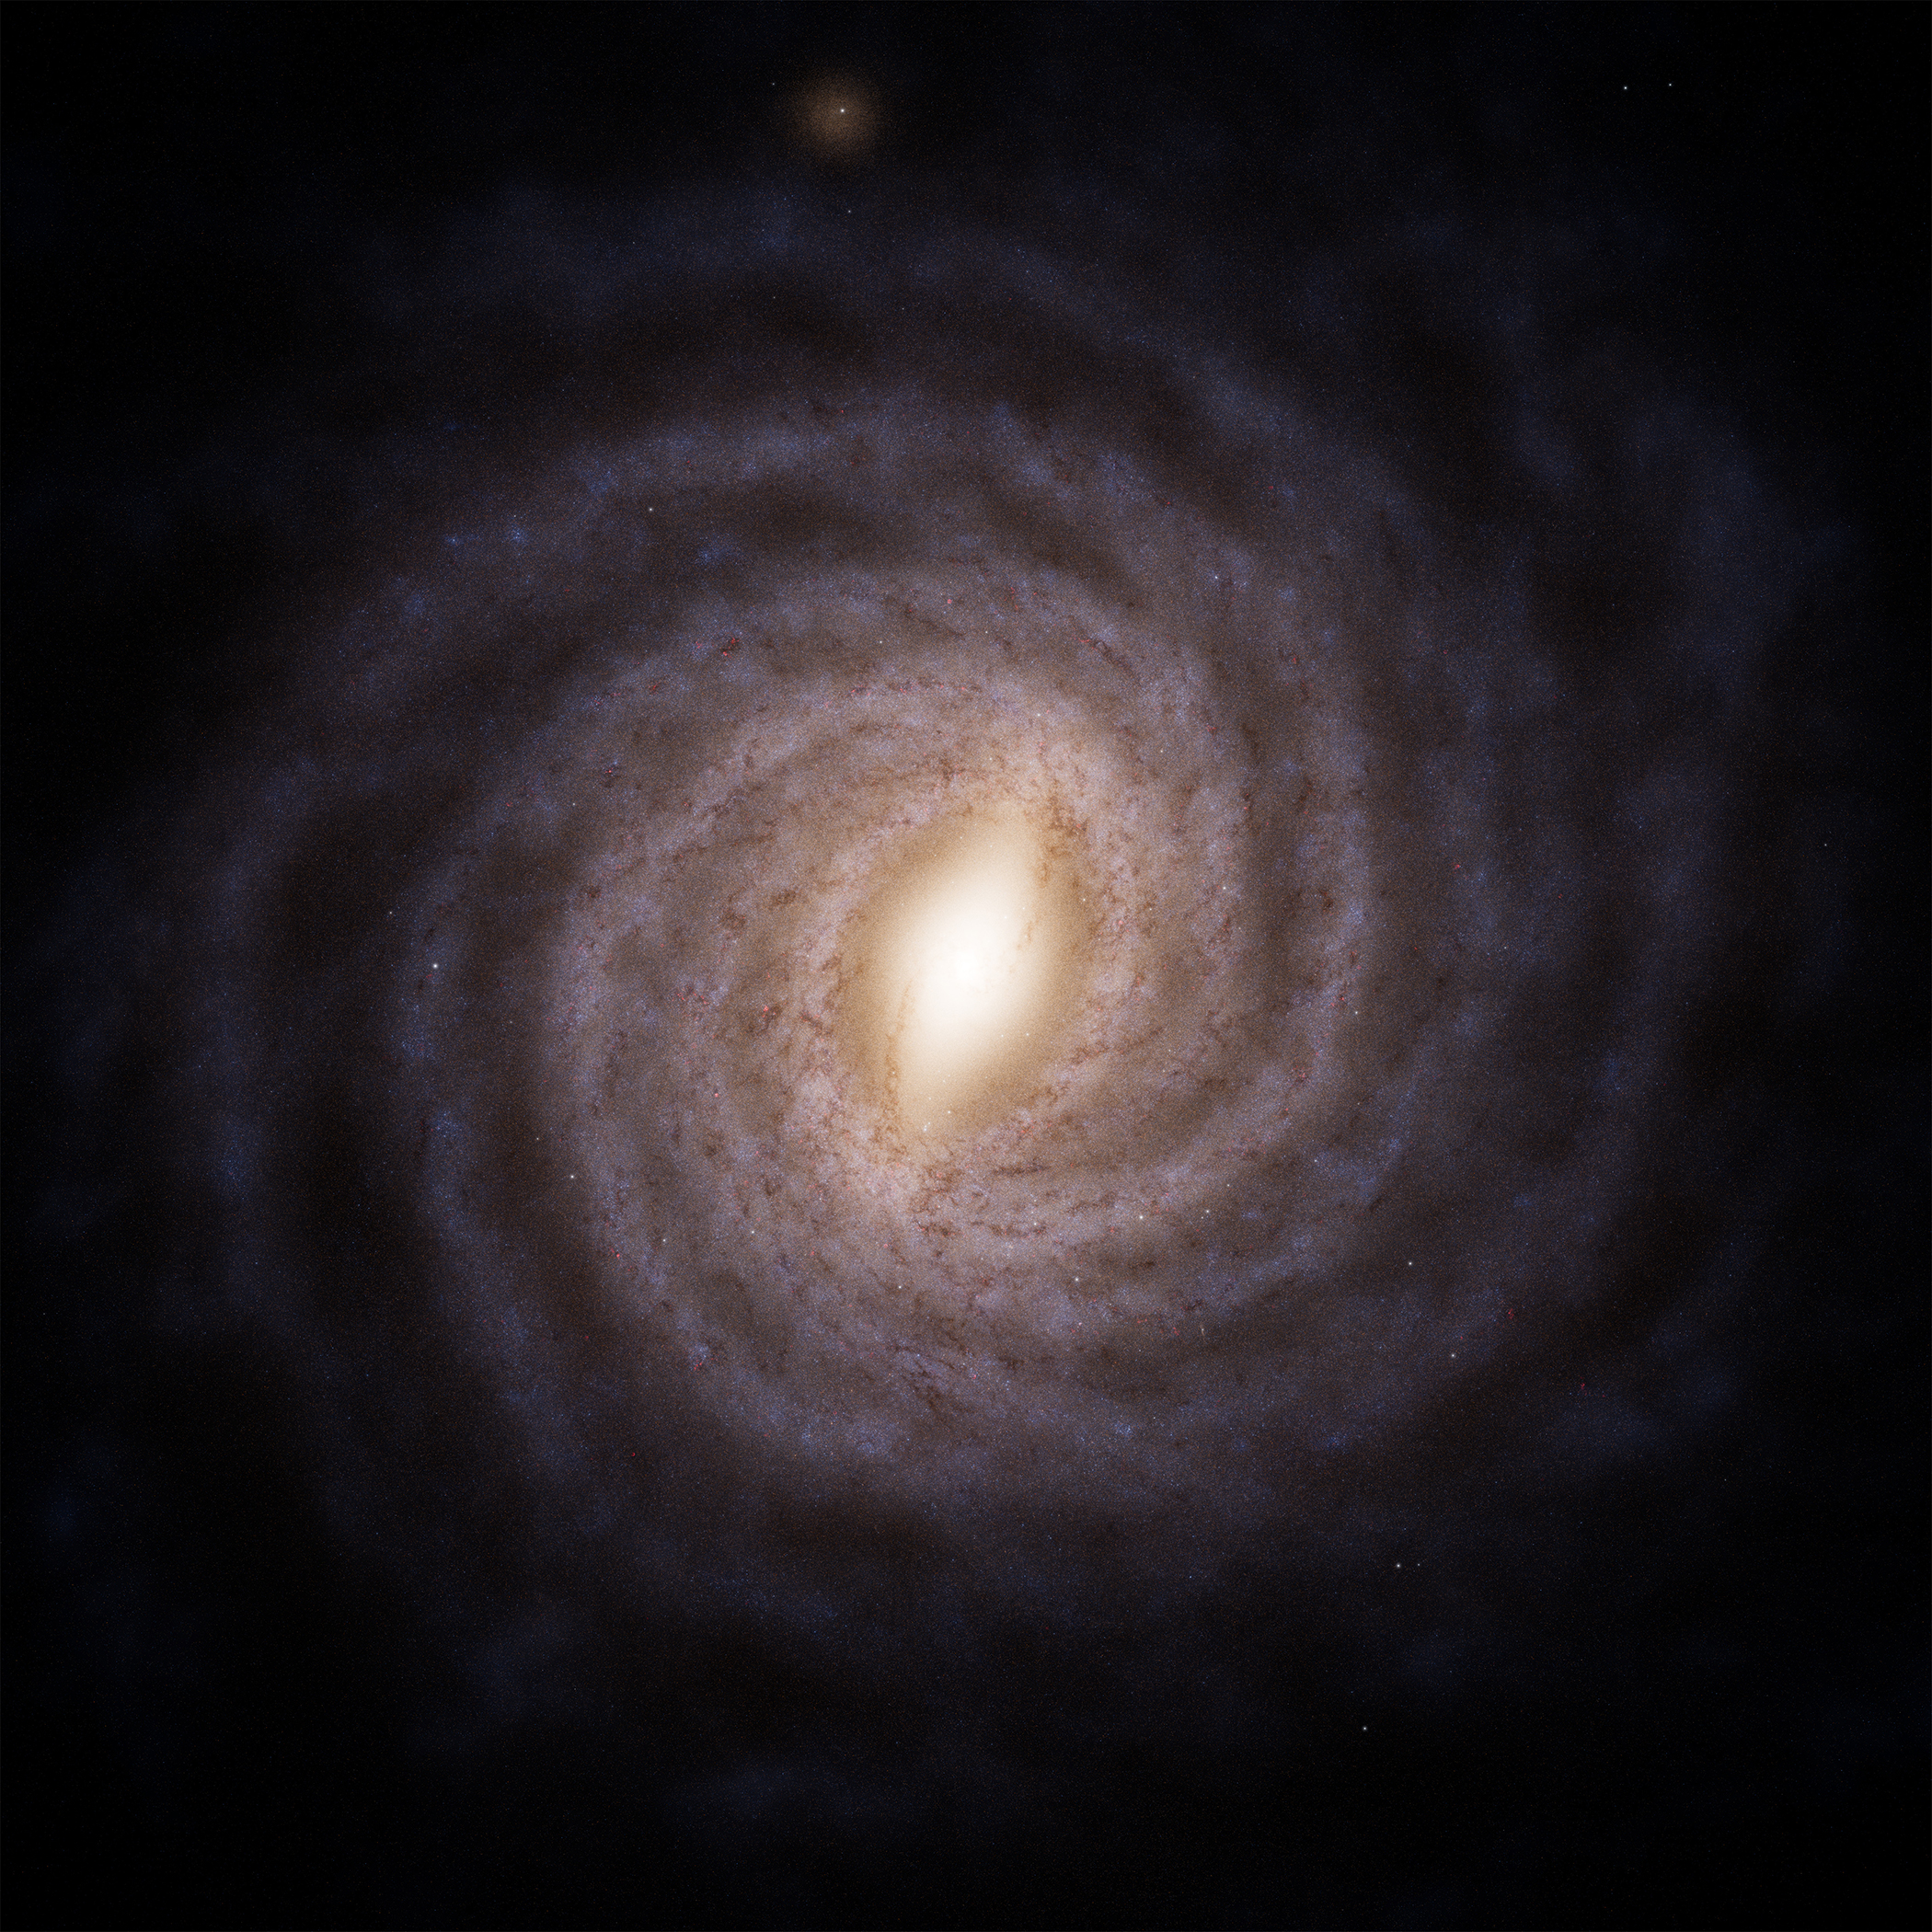
\includegraphics[width=\linewidth]{milky-way.jpg}};
  \begin{scope}[x={(map.south east)},y={(map.north west)}]
   \tikzset{tag/.style={font=\sffamily\fontsize{7}{8}\selectfont,text=white,fill=black,fill opacity=.65,text opacity=1,inner sep=3pt,align=left}}
   \draw[white,opacity=.65,line width=.4pt] (.49,.5)--(.58,.56);
   \node[tag,anchor=west] at (.57,.58) {Galactic centre};
   \draw[gold!65!white,dashed,line width=.7pt] (.5,.5) circle[radius=.205];
   \node[tag] at (.26,.47) {Sun's orbit\\$R_0\approx8.2$ kpc};
   \draw[-{Stealth[length=2mm]},gold!65!white,line width=1pt] (.5,.295) arc[start angle=270,end angle=236,radius=.205];
   \draw[-{Stealth[length=2mm]},gold!65!white,line width=1pt] (.386,.330) arc[start angle=236,end angle=204,radius=.205];
   \fill[gold!65!white] (.5,.295) circle[radius=.008];
   \fill[orange!70!white] (.386,.330) circle[radius=.008];
   \fill[cyan!65!white] (.313,.417) circle[radius=.008];
   \node[tag,anchor=north] at (.53,.265) {A / today};
   \node[tag,anchor=north east] at (.40,.30) {B / future};
   \node[tag,anchor=east] at (.29,.385) {C / later};
   \node[tag] at (.71,.78) {Perseus arm};
   \node[tag] at (.72,.65) {Sagittarius--Carina};
   \node[tag] at (.30,.64) {Scutum--Centaurus};
   \node[tag,anchor=west] at (.62,.32) {Local arm};
   \node[tag,anchor=west] at (.04,.92) {FACE-ON RECONSTRUCTION\\Observer epochs are schematic};
   \node[tag,anchor=south west] at (.04,.045) {Spiral structure is not a rigid track.\\The surrounding stars move too.};
  \end{scope}
 \end{tikzpicture}
 \figcap{A new annotated rendering of the original question. ESA/Gaia/DPAC, Stefan Payne-Wardenaar reconstruction [1], adapted with vector labels. Epoch positions, orbit and arm-name placement are schematic, not fitted boundaries or a predicted future sky.}
\end{minipage}

\takeaway{Working answer}{Relative motion can help or hinder a particular observation. In the selected century experiment, the imaging-accessibility sum changes by only \textbf{+0.0307\%}; the specified instrument-improvement scenario changes it much more. Neither result forecasts life or a number of discoveries.}
\vspace{5pt}
\source{Project, full methods, original discussion note and reproducible code: \href{https://biswajit1999.github.io/moving-observer/}{biswajit1999.github.io/moving-observer/}. This is a discussion report inviting expert criticism, not a claim of a new physical law.}
